
\subsection{Sploty}
% DICTIONARY;link;splot;-
% GLOSSAIRE;un entrelacs;splot;-
% DICTIONARY;component;ogniwo splotu;-
% GLOSSAIRE;composante/boucle;ogniwo splotu;-
\begin{definition}[splot, ogniwo]
\index{splot}%
    Sumę parami rozłącznych węzłów
    \begin{equation}
        L = K_1 \sqcup K_2 \sqcup \ldots K_n
    \end{equation}
    nazywamy splotem, a~składniki $K_i$ -- ogniwami splotu.
\end{definition}

Przez analogię do węzłów mówimy, że dwa sploty są takie same, jeśli jeden jest obrazem drugiego przez zachowujący orientację homeomorfizm $\R^3 \to \R^3$.
To oczywiste, że liczba ogniw jest niezmiennikiem splotów.
Później podamy mniej oczywiste niezmienniki.

\begin{example}[niesplot]
\index{niesplot}%
    Splot zadany w przestrzeni $\R^3$ parametrycznie
    \begin{equation}
        \bigcup_{k=1}^n \{(\sin \theta, \cos \theta, k) : \theta \in [0, 2\pi]\}
    \end{equation}
    nazywamy niesplotem i oznaczamy $U_n$.
\end{example}
    
\begin{example}
\index{splot!Hopfa}%
\index[persons]{Hopf, Heinz}%
    Splot Hopfa (rys. \ref{small_links_diagram}a), najprostszy nietrywialny splot. Ma dwa ogniwa.
\end{example}

\begin{remark}[Heinz Hopf]
    Matematyk niemiecki urodzon w 1894 roku w Gräbschen (obecnie część Wrocławia); zmarł w 1971 roku w Zurychu, Szwajcarii.
    Głównym wynikiem jego pracy doktorskiej z~1925 roku było, że każda jednospójna zupełna 3-rozmaitość Riemanna o~stałej krzywiźnie sekcyjnej jest globalnie izometryczna do przestrzeni euklidesowej, sferycznej lub hiperbolicznej.
    Był pionierem topologii algebraicznej.
    W~1931 roku prowadził badania nad tzw. rozwłóknieniem: odwzorowaniem $S^3 \to S^2$ takim, że przeciwobrazy punktów są okręgami wielkimi na 3-sferze.
    Podczas tych badań zajmował się splotem nazywanym teraz splotem Hopfa.
\end{remark}

\begin{example}
\index{splot!Whiteheada}%
\index[persons]{Whitehead, John}%
    Splot Whiteheada (rys. \ref{small_links_diagram}b).
\end{example}

\begin{remark}[John Henry Constantine Whitehead]
    Matematyk brytyjski urodzon w 1903 roku w~Madrasie, Indiach; zmarł w 1960 roku w Princeton, New Jersey.
    Był jednym z założycieli teorii homotopii, podał definicję CW-kompleksów.
    Próbował udowodnić hipotezę Poincarégo, ale popełnił błąd twierdząc, że nie istnieje ściągalna otwarta 3-rozmaitość, która nie jest homeomorficzna z $\R^3$.
    W 1935 roku sam wskazał taką rozmaitość, do jej konstrukcji wykorzystując splot Whiteheada.
\end{remark}

\begin{comment}
    {\setlength{\intextsep}{4pt plus 2pt minus 2pt}
    \begin{figure}[H]
        \centering
        \begin{minipage}[b]{.3\linewidth}
            \centering
            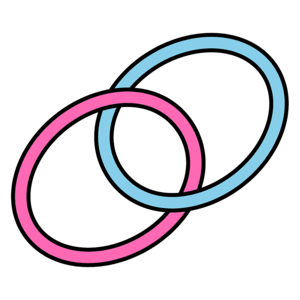
\includegraphics[height=0.6\linewidth]{../data/links/2_2_1.png}
            \subcaption{splot Hopfa}
        \end{minipage}\,\,
        \begin{minipage}[b]{.3\linewidth}
            \centering
            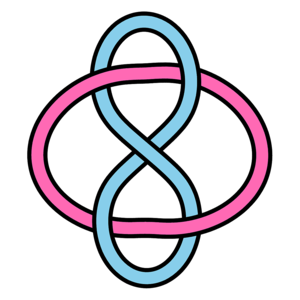
\includegraphics[height=0.6\linewidth]{../data/links/5_2_1.png}
            \subcaption{splot Whiteheada}
        \end{minipage}\,\,
        \begin{minipage}[b]{.3\linewidth}
            \centering
            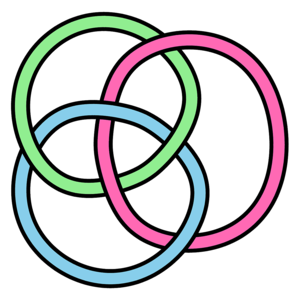
\includegraphics[height=0.6\linewidth]{../data/links/6_3_2.png}
            \subcaption{pierścienie Boromeuszy}
            \index{pierścienie Boromeuszy}%
        \end{minipage}
        \caption[small-links]{Sploty o małej liczbie skrzyżowań}
        \label{small_links_diagram}
    \end{figure}
    }
\end{comment}


\subsubsection{Sploty rozszczepialne}
Aby wytłumaczyć, czemu trzeci splot z rysunku \ref{small_links_diagram} jest interesujący, potrzebujemy zdefiniować sploty rozszczepialne.

% DICTIONARY;splittable;rozszczepialny;splot
\begin{definition}[rozszczepialność]
\index{splot!rozszczepialny}%
    Jeżeli splot $L$ można zanurzyć w przestrzeni $\R^3$ tak, że niektóre jego ogniwa będą leżeć nad pewną rozłączną ze splotem płaszczyzną, zaś pozostałe pod nią, to powiemy, że splot $L$ jest rozszczepialny.
\end{definition}

Liczbę nierozszczepialnych splotów pierwszych kopiujemy z bazy danych LinkInfo \cite{linkinfo24}:
\renewcommand*{\arraystretch}{1.4}
\footnotesize
\begin{longtable}{lcccccccccccc}
    \hline
    \textbf{skrzyżowania} & 0 & 1 & 2 & 3 & 4 & 5 &  6 &  7 &  8 & 9 & 10 & 11 \\ \hline \endhead
    sploty pierwsze, nierozszczepialne & 0 & 0 & 1 & 0 & 1 & 1 & 6 & 9 & 29 & 83 & 287 & 1007 \\
    (w tym) alternujące & 0 & 0 & 1 & 0 & 1 & 1 & 5 & 7 & 21 & 55 & 174 & 548 \\
    (w tym) niealternujące & 0 & 0 & 0 & 0 & 0 & 0 & 1 & 2 & 8 & 28 & 113 & 459 \\
    \hline
\end{longtable}
\normalsize

W bazie liczb OEIS trafiliśmy tylko na ciąg \href{https://oeis.org/A086826}{A086826} opisujący liczbę nierozszczepialnych pierwszych i złożonych węzłów i splotów, na przykład $a_5 = 4$, bo mamy dwa węzły pierwsze, splot Whiteheada oraz trójlistnik spleciony z~niewęzłem.
Słowa ,,skrzyżowanie'' , ,,alternujący'' oraz ,,pierwszy'' definiujemy w~przyszłości, będą to odpowiednio definicje \ref{def:crossing}, \ref{def:alternating_link} i \ref{def:prime_knot}.
\index{węzeł!alternujący}%
\index{węzeł!pierwszy}%
\index{skrzyżowanie}%
Książka ma nieliniową budowę i należy przeczytać ją co najmniej dwa razy.

Pewne kryteria rozszczepialności konkretnych splotów znaleźć można u Kawauchiego \cite[s. 36-38]{kawauchi1996}.
% przepisać, a jeśli za trudne, to może chociaż szkic?




\subsubsection{Sploty Brunna}
\index{splot!Brunna|(}%
Hermann Brunn \cite{brunn1892} rozpatrywał w 1892 roku (a więc zanim jeszcze teoria węzłów przyszła na świat!) nierozszczepialne sploty, które po usunięciu dowolnego ogniwa stają się niesplotami.
\index[persons]{Brunn, Hermann}%
W~czasopiśmie Delta, nr 01/2011, przeczytaliśmy, że Rolfsen zaproponował nazywać je splotami Brunna i~tak też będziemy robić.
Najprostszym splotem Brunna są posiadające trzy ogniwa pierścienie Boromeuszy ($6_2^3$ w notacji Alexandera-Briggsa, \texttt{L6a4} w notacji Thistlethwaite'a).
\index{pierścienie Boromeuszy}%
Pokażemy na stronie \pageref{boromean_not_splittable}, że pierścienie Boromeuszy nie mają nietrywialnych trójkolorowań, więc nie mogą być niesplotem.

Pierścienie Boromeuszy są alternujące, hiperboliczne i drzewiaste.
\index{węzeł!alternujący}%
\index{węzeł!hiperboliczny}%
\index{węzeł!drzewiasty}%
% DICTIONARY;arborescent;drzewiasty;węzeł
% TODO: jak jest arborescent po francusku?
Ich nazwa pochodzi od lombardzko-piemonckiego rodu kupieckiego, bankierskiego i arystokratycznego, z którego wywodziło się wielu kardynałów.
Herb tego rodu zawierał splecione ze sobą trzy okręgi.
Jest niemożliwe, by wykonać model przestrzenny tego splotu przy użyciu okrągłych pierścieni.
Zamiast tego można użyć na przykład elips.

Z dokładnością do homotopii sploty Brunna zostały sklasyfikowane przez Milnora \cite{milnor1954}, ale ponieważ ta książka nie tłumaczy, czym są $\mu$-niezmienniki Milnora, nie możemy dzisiaj wytłumaczyć, jak tego dokonał.
\index[persons]{Milnor, John}%
\index{splot!Brunna|)}%




\subsubsection{Sploty alternujące}

Zazwyczaj do zdefiniowania splotów alternujących potrzebne są najpierw diagramy.
% Zanim opowiemy, jak dotąd przebiegała klasyfikacja węzłów o małej liczbie skrzyżowań, zdefiniujemy klasę splotów ze specjalnymi diagramami.

% DICTIONARY;alternating;alternujący;węzeł
\begin{definition}[splot alternujący]
\label{def:alternating_link}%
\index{węzeł!alternujący}%
    Niech $D$ będzie diagramem splotu $L$.
    Jeżeli podczas poruszania się wzdłuż każdego ogniwa naprzemiennie mijamy podskrzyżowania oraz nadskrzyżowania, to diagram nazywamy alternujący.
    
    Splot $L$ jest alternujący, jeśli posiada alternujący diagram $D$s.
\end{definition}

Około 1961 roku Ralph Fox zapytał \emph{,,What is an alternating knot?''}.
\index[persons]{Fox, Ralph}%
Szukano takiej definicji węzła alternującego, która nie odnosi się bezpośrednio do diagramów, aż w~2015 roku Greene \cite{greene2017} podał geometryczną charakteryzację: nierozszczepialny splot w $S^3$ jest alternujący wtedy i~tylko wtedy, gdy ogranicza dodatnią oraz ujemną określoną powierzchnię rozpinającą.
\index[persons]{Greene, Joshua}%

\begin{remark}[Ralph Hartzler Fox]
    Matematyk amerykański urodzon w Morrisville, Pensylwanii w~1913 roku; zmarł w Filadelfii, tamże w 1973 roku.
    Był promotorem Johna Milnora, Lee Neuwirtha (o~których jeszcze wspomnimy!) i 23 innych osób, o których nie wspomnimy.
    Oprócz tego nadzorował pracę licencjacką Kennetha Perko.
    Zawdzięczamy mu spopularyzowanie $n$-kolorowania na koledżu Haverford w 1956 roku, podanie nowego sposobu na znalezienie wielomianu Alexandera przy użyciu rachunku różniczkowego Foxa oraz niektóre terminy teorii węzłów uzywane po dziś dzień: węzeł plastrowy, węzeł taśmowy, okrąg i powierzchnia Seiferta.
\end{remark}

Nie ma zwartego wzoru na liczbę splotów alternujących, ale wiemy, że rośnie co najmniej wykładniczo względem liczby skrzyżowań:

\begin{proposition}
\index{supeł}%
    Niech $a_n$ oznacza liczbę supłów o~$n$ skrzyżowaniach, które są alternujące oraz pierwsze.
    Wtedy
    \begin{equation}
        a_n \sim \frac{3c_1 \lambda^{n-3/2}}{4\sqrt{\pi n^{5}}},
    \end{equation}
    gdzie zarówno $c_1$, pierwszy współczynnik rozwinięcia Taylora funkcji $\Phi(\eta)$ zdefiniowanej w \cite{sundberg1998}, jak i $\lambda$ są jawnie znanymi stałymi:
    \begin{align}
        c_1 & = \sqrt{\frac{5^7 \cdot (21001 + 371 \sqrt{21001})^3}{2 \cdot 3^{10} \cdot (17 + 3\sqrt{21001})^5}} \\
        \lambda & = \frac {1}{40} (101 + \sqrt{21001})
    \end{align}
    Niech $A_n$ oznacza liczbę pierwszych, alternujących splotów o $n$ skrzyżowaniach.
    Wtedy $A_n \approx \lambda^n$, dokładniej: jeśli $n \ge 3$, to
    \begin{equation}
        \frac{a_{n-1}}{16n - 24} \le A \le \frac{a_n - 1}{2}.
    \end{equation}
\end{proposition}

Węzły pierwsze i~supły pojawiają się odpowiednio w definicjach \ref{def:prime_knot}, \ref{def:tangle}.

\begin{proof}[Niedowód]
\index[persons]{Sundberg, Carl}%
\index[persons]{Thistlethwaite, Morwen}%
    Zamiast przedstawić dowód albo chociaż jego szkic, wymienimy trzy narzędzia użyte przez Sundberga, Thistlethwaite'a \cite{sundberg1998}:
    algebraiczną metodę Conwaya znajdowania splotów,
    wynik Tuttego dotyczącego liczby ukorzenionych $c$-sieci
    oraz (wtedy już udowodnioną) hipotezę Taita.
\index[persons]{Conway, John}%
\index[persons]{Tutte, William}%
\index{hipoteza!Taita}%
\end{proof}

\begin{proposition}
    Niech $a_n$ oznacza liczbę supłów o~$n$ skrzyżowaniach, które są alternujące oraz pierwsze.
    Wtedy funkcja tworząca $f(z) = \sum_n a_n z^n$ spełnia równanie
    \begin{equation}
    f(1+z) - f(z)^2 - (1+f(z))q(f(z)) -z - \frac{2z^2}{1-z} = 0,
    \end{equation}
    gdzie $q(z)$ jest pomocniczą funkcją
    \begin{equation}
        q(z) = \frac{2z^2 - 10z - 1 + \sqrt{(1-4z)^3}} {2(z+2)^3} - \frac{2}{1+z} -z + 2.
    \end{equation}
\end{proposition}

Powyższa ciekawostka także pochodzi z cytowanej wcześniej pracy \cite{sundberg1998}.



